% 第 14 章 Creating Routes
\bichapter{创建布线}{Creating Routes}
\label{chap:gui-route}

IC Compiler II GUI 提供交互界面与程序化接口，用来快速创建布线（route）。使用 Create Route 工具，可在设计中的管脚（pin）、端口（port）以及其他布线形状（route shape）之间，为一根或多根线网（net）或线束（bundle）布线。与 Create Route 工具类似，Create RDL 工具用于为单根线网布线，在再分布层（redistribution layer，RDL）或其他金属层上创建正交布线与 45 度布线。\cmd{create\_trunk}、\cmd{create\_trunk\_pin\_to\_pin} 与 \cmd{create\_trunk\_pin\_to\_trunk} 命令根据命令行选项，在指定线网上创建布线段。

下列主题说明如何使用 GUI 创建布线：
\begin{itemize}
  \item 交互创建布线
  \item 对布线做交互式设计规则检查
  \item 用 Tcl 命令或 GUI 创建布线主干
  \item 在布线上添加缓冲器
  \item 估算点到点电阻
\end{itemize}

% ============================================================
\section{交互创建布线}
\subsection*{Creating Routes Interactively}

Create Route 工具可以交互地为一根或多根线网或线束布线。工具选项指定布线的创建方式。工具支持避开阻挡（blockage），并提供设计规则检查（design rule checking，DRC）反馈，帮助创建高质量、无违例（violation）的布线与连接。吸附（snapping）、自动对齐（auto-alignment）与自动焊接（auto-welding）用于把新布线快速接到管脚或已有布线上。线束布线（bundle routing）支持同时为多条信号布线。

\subsection{启动 Create Route 工具}
\subsubsection*{Starting the Create Route Tool}

要启动 Create Route 工具，采用下列任一方式：
\begin{itemize}
  \item 单击 Create Route 按钮
  \item 在菜单中选择 \textbf{Create > Route}
  \item 按 Shift+R
\end{itemize}

工具启动并显示 Create Route 工具栏。

\subsection{指定层、线宽、节距与端帽样式}
\subsubsection*{Specifying Layer, Width, Pitch, and End-Cap Style}

Create Route 工具在工具栏上提供设置与选项，用来指定布线的层、线宽、节距（pitch）与端帽样式（end-cap style），如图~\ref{fig:gui-152} 所示。单击工具栏上的 More、DRC 或 Snap 按钮，还可以使用其他设置。

\begin{figure}[htbp]
\centering
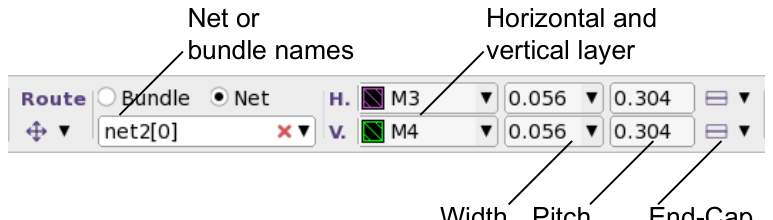
\includegraphics[width=0.92\textwidth]{gui-fig-152.png}
\caption{层名、线宽、节距与端帽设置}
\label{fig:gui-152}
\end{figure}

可用下列任一方法指定线网或线束的层名、线宽与节距：
\begin{itemize}
  \item 在输入框中输入线网名或线束名。工具把水平层与垂直层设为用于布线的最低金属层。
  \item 在启动 Create Route 工具之前选择一个管脚，以便推断线网名。工具根据所选管脚设置层、线宽等参数。
  \item 在工具栏 Auto 部分选择 Net，然后单击一条已有布线，从该布线推断线网名。若要从已有布线推断层、线宽或端帽样式，在 Auto 部分选择对应选项。
  \item 在工具栏的 More 设置面板中启用 Connect to pin by layer，并指定层名。自动连接到管脚时，工具使用指定的层，除非这些管脚是布线的起点或终点。
\end{itemize}

\subsection{在管脚之间创建布线}
\subsubsection*{Creating Routes Between Pins}

为一组管脚创建布线：
\begin{enumerate}
  \item 选择要布线的线网的源管脚或目标管脚。
  \item 按 Shift+R，或单击 Create Route 工具按钮，启动 Create Route 工具。
  \item 在工具栏单击 More，并在 Advanced options 部分选择 Extend first 与 Extend last。
\end{enumerate}

\begin{figure}[htbp]
\centering
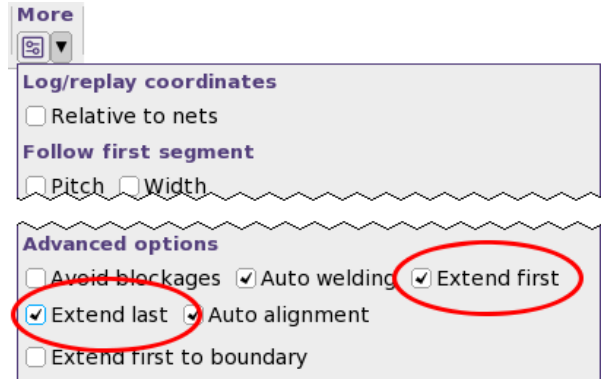
\includegraphics[width=0.92\textwidth]{gui-fig-153.png}
\caption{管脚到管脚连接布线的设置}
\label{fig:gui-153}
\end{figure}

\begin{enumerate}
  \setcounter{enumi}{3}
  \item 把指针放在靠近所选管脚的布线路径上并单击鼠标，开始绘制布线，如图~\ref{fig:gui-154} 中的（A）所示。
\end{enumerate}

\begin{figure}[htbp]
\centering
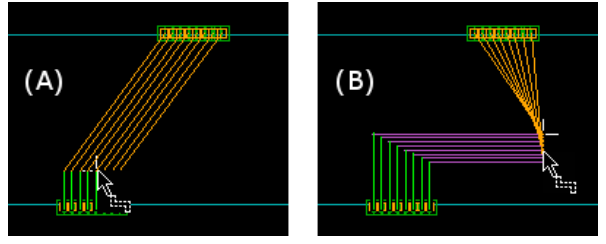
\includegraphics[width=0.92\textwidth]{gui-fig-154.png}
\caption{从所选管脚布线}
\label{fig:gui-154}
\end{figure}

\begin{enumerate}
  \setcounter{enumi}{4}
  \item 单击以创建一个拐角，然后沿正交方向移动鼠标指针，如图中的（B）所示。按需要重复本步，以创建更多布线段。
  \item 把鼠标指针移到目标管脚附近，直到工具显示完成的布线，如图~\ref{fig:gui-155} 中的（C）所示。
\end{enumerate}

\begin{figure}[htbp]
\centering
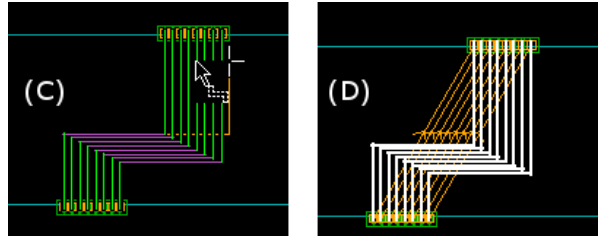
\includegraphics[width=0.92\textwidth]{gui-fig-155.png}
\caption{完成布线}
\label{fig:gui-155}
\end{figure}

\begin{enumerate}
  \setcounter{enumi}{6}
  \item 按 Enter 键，或单击鼠标右键并在上下文菜单中选择 Apply，完成布线。工具完成的布线如图中的（D）所示。
\end{enumerate}

\subsection{按第一段套用布线段的线宽与间距}
\subsubsection*{Applying Route Segment Width and Spacing Based on the First Segment}

要使全部布线段采用与第一段相同的线宽与间距，在工具栏单击 More，并在 Follow first segment 部分启用 Pitch 与 Width。启用后，工具使后续全部布线段与第一段一致，如图~\ref{fig:gui-156} 所示。

\begin{figure}[htbp]
\centering
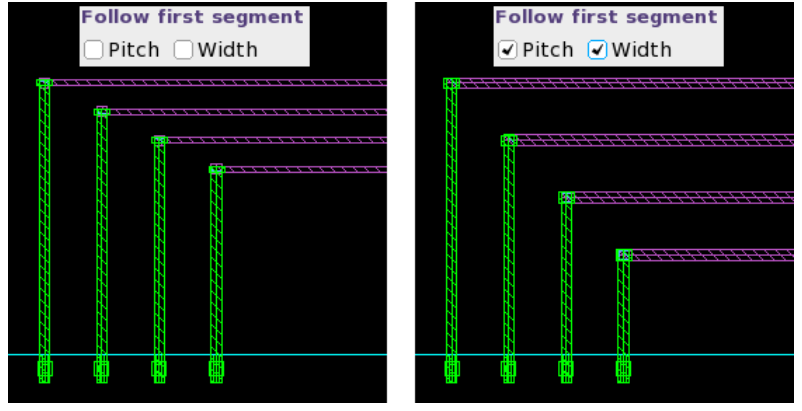
\includegraphics[width=0.92\textwidth]{gui-fig-156.png}
\caption{跟随第一段}
\label{fig:gui-156}
\end{figure}

\subsection{创建偏离轨道的布线}
\subsubsection*{Creating Off-Track Routes}

要创建偏离轨道（off-track）的布线段，在工具栏单击 More，并在 Snap to track 部分关闭 First net 与 Every net。默认启用 First net，第一段布线创建在布线轨道（track）上。这些选项如图~\ref{fig:gui-157} 所示。

\begin{figure}[htbp]
\centering
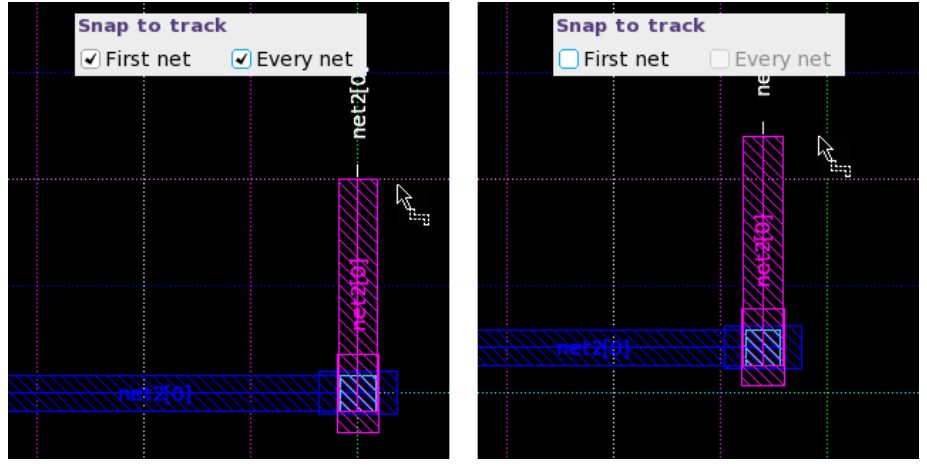
\includegraphics[width=0.92\textwidth]{gui-fig-157.png}
\caption{吸附到轨道}
\label{fig:gui-157}
\end{figure}

\subsection{在所绘路径的上方或下方创建后续布线}
\subsubsection*{Creating Successive Routes Above or Below the Drawn Path}

Create Route 工具从线束或线网名输入框中的第一根线网开始，沿用鼠标绘制的路径创建布线。后续线网与第一根线网平行创建；方向由 More 设置面板中 When starting use 部分的 Low end 与 High end 决定。

下面的示例用 \cmd{create\_bundle} 命令创建名为 \cmd{bundle4} 的线束，并用它为四根线网布线：
\begin{lstlisting}
icc2_shell> create_bundle -name {bundle4} \
    {net2[127] net2[126] net2[125] net2[124]}
\end{lstlisting}

列表中的第一根线网是 \cmd{net2[127]}，它沿用鼠标绘制的路径创建。默认情况下，后续线网创建在 \cmd{net2[127]} 的上方或右侧，如图~\ref{fig:gui-158} 左侧所示。黄色高亮表示用鼠标绘制布线时的路径。

\begin{figure}[htbp]
\centering
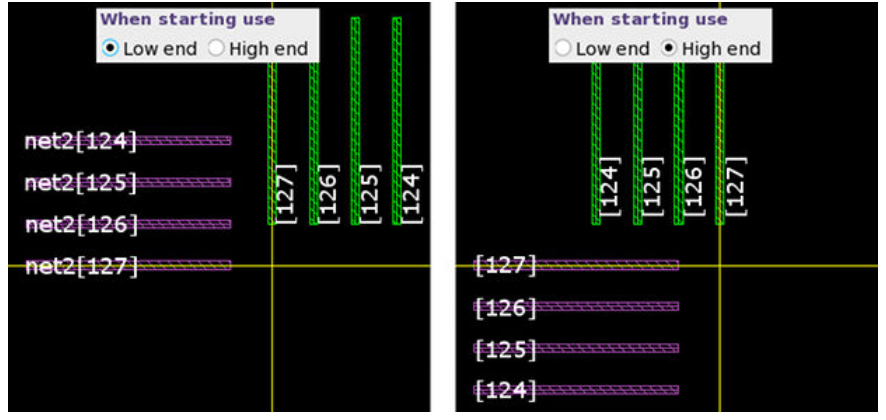
\includegraphics[width=0.92\textwidth]{gui-fig-158.png}
\caption{低端与高端布线选项}
\label{fig:gui-158}
\end{figure}

要使后续布线位于鼠标路径的下方或左侧，在工具栏单击 More 并选择 High end。工具创建的布线如图~\ref{fig:gui-158} 右侧所示。

\subsection{更改正交布线的线网顺序}
\subsubsection*{Changing the Route Ordering for Orthogonal Routes}

创建正交布线时，Create Route 工具支持多种线网排序方式。默认情况下，工具保持线网顺序，并在创建新布线段时避免布线重叠。要在创建正交布线时反转布线顺序，单击 More，并在 When turning 部分启用 Switch ends。要在拐弯处把布线错开，启用 Switch ends，并把 Skip count 设为大于 1 的值。设置这些选项后的布线结果如图~\ref{fig:gui-159} 所示。

\begin{figure}[htbp]
\centering
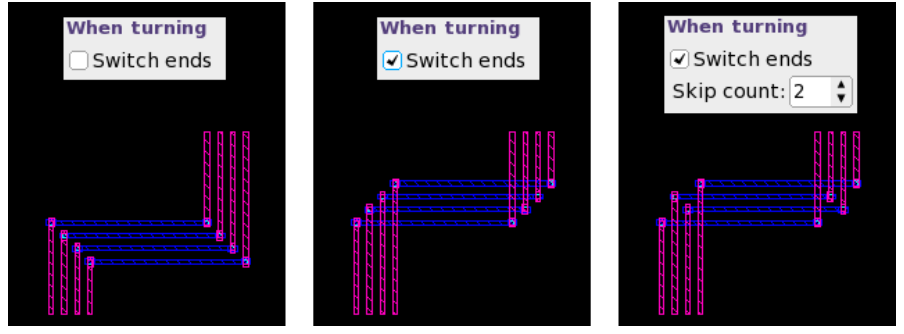
\includegraphics[width=0.92\textwidth]{gui-fig-159.png}
\caption{布线拐弯样式}
\label{fig:gui-159}
\end{figure}

\subsection{显示布线引导飞线与标注}
\subsubsection*{Displaying Route Guidance Flylines and Annotations}

Create Route 工具显示飞线（flyline）与其他引导，帮助创建布线。启动 Create Route 工具并输入线网名后，工具在布线的管脚与端口之间显示一条静态飞线（static flyline）。开始布线后，工具再加入一条动态飞线（dynamic flyline），显示到最近管脚连接的最短路径；移动鼠标创建布线段时，动态飞线随之更新。布线完成后，动态飞线被去掉。默认情况下，工具在布线的管脚与端口之间显示飞线，并在布线中的端口上显示端口引导标记（port guidance marker）。

要隐藏飞线与端口引导标记，单击 More，并在面板 Show 部分取消选择 Port Guidance 与 Flylines。要显示已有布线，以及随布线段创建而动态更新的当前布线电阻值，在面板中选择 Routes 与 Resistance。面板中的选项以及与这些选项对应的版图标注如图~\ref{fig:gui-160} 所示。

\begin{figure}[htbp]
\centering
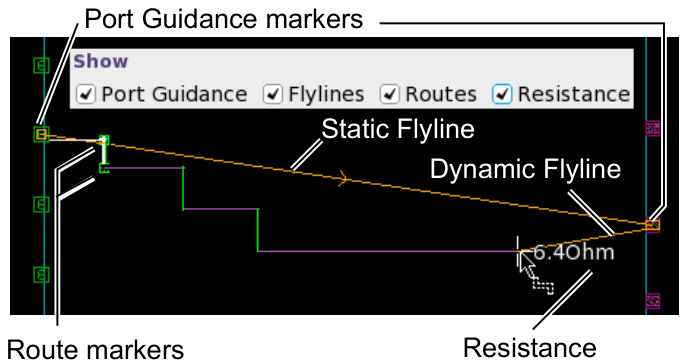
\includegraphics[width=0.92\textwidth]{gui-fig-160.png}
\caption{显示飞线与其他标注}
\label{fig:gui-160}
\end{figure}

\subsection{避免连接到已有布线}
\subsubsection*{Preventing Connections to Existing Routes}

要避免工具在跨越同一线网的布线时自动创建通孔（via），单击 More，并在面板 Advanced options 部分取消选择 Auto welding。更改该选项后的布线结果如图~\ref{fig:gui-161} 所示。

\begin{figure}[htbp]
\centering
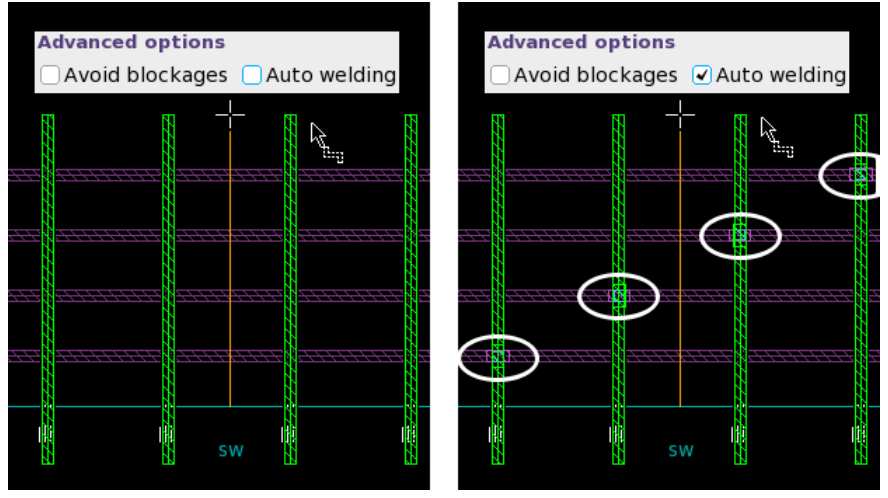
\includegraphics[width=0.92\textwidth]{gui-fig-161.png}
\caption{自动焊接}
\label{fig:gui-161}
\end{figure}

\subsection{设置搜索距离并指定搜索层}
\subsubsection*{Setting a Search Distance and Specifying Layers to Search}

Create Route 工具会自动连接到位于当前鼠标位置搜索距离（search distance）之内的管脚。若已启用 Auto welding，而又不希望工具连接到管脚，单击 More，并把 Welding and extend options 部分中 Search distance 框的值设为 0。若希望工具连接到更远的管脚，增大该距离，使工具能搜索离布线更远的管脚。同一组管脚、沿黄色高亮绘制的同一条布线，在不同搜索距离下的版图结果如图~\ref{fig:gui-162} 所示。

\begin{figure}[htbp]
\centering
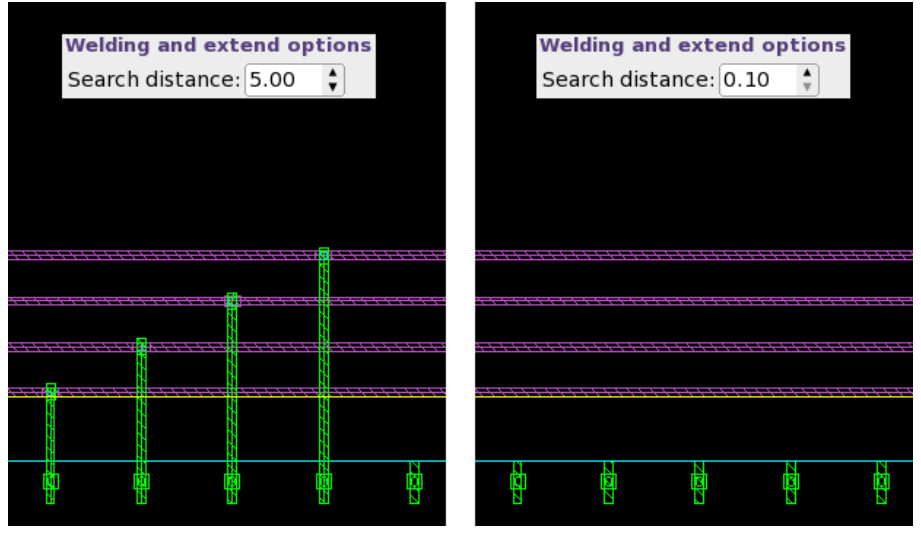
\includegraphics[width=0.92\textwidth]{gui-fig-162.png}
\caption{搜索距离}
\label{fig:gui-162}
\end{figure}

工具在全部布线层上搜索连接。要把搜索限制在相邻层，单击 More，并在面板 Welding and extend options 部分选择 Search Layers: Adjacent。选中后，工具只连接到与当前布线层相邻的一层上的管脚。要指定搜索的层范围，在同一部分选择 Specified，并在层列表框中选择一层或多层。

\subsection{指定其他焊接与连接选项}
\subsubsection*{Specifying Other Welding and Connection Options}

Create Route 工具还提供其他选项，用来指定与已有布线或管脚的连接。
\begin{itemize}
  \item \textbf{Ignore pin access direction}：选中后，工具自动把布线连接到管脚，不考虑管脚接入方向（pin access direction）。默认会考虑管脚接入方向。
  \item \textbf{Skip PG nets}：选中后，避免连接到电源地（power and ground，PG）线网。当这些线网用于线网屏蔽（net shielding）时，用本选项跳过与地线网的连接。
  \item \textbf{Honor via to via spacing}：选中后，工具遵守同一线网的通孔到通孔间距（via-to-via spacing）规则。
  \item \textbf{No via on pin}：连接到管脚时避免插入通孔。
  \item \textbf{Adjust to pin width}：选中后，若线宽小于管脚宽度，工具把布线宽度设为管脚宽度。默认不选中本选项，线宽在工具栏中指定。若线宽大于管脚宽度，则采用管脚宽度作为线宽。
  \item \textbf{Align with pin center}：取消选择后，工具把连接线与最近的平行管脚边对齐，或把线延伸到平行管脚边的边界之内。轨道吸附与间距要求可能影响最终的线位置。默认选中本选项，工具在可能时把布线与管脚包围盒（bounding box）的中心对齐。当管脚宽于连接线时，工具可能把线移离中心，以遵守轨道吸附与间距设置。
\end{itemize}

\subsection{创建 45 度布线与 RDL 布线}
\subsubsection*{Creating 45-Degree and RDL Routes}

Create RDL 工具支持 Create Route 工具的许多相同功能。此外，Create RDL 工具可以在再分布层上创建 RDL 布线，并在单一金属层上创建一般的 45 度布线，如图~\ref{fig:gui-163} 所示。

\begin{figure}[htbp]
\centering
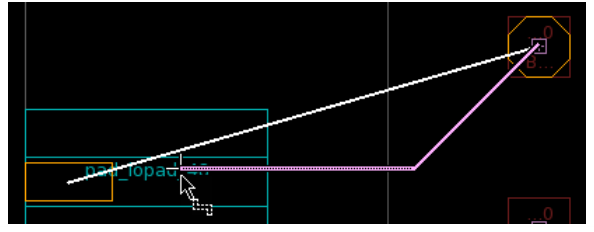
\includegraphics[width=0.92\textwidth]{gui-fig-163.png}
\caption{Create RDL 工具}
\label{fig:gui-163}
\end{figure}

用 Create RDL 工具创建 45 度布线：
\begin{enumerate}
  \item 在菜单中选择 \textbf{Create > RDL}，或单击 Create RDL 按钮，启动 Create RDL 工具。
  \item 在线网名输入框中输入要布线的线网或线束名。
  \item （可选）单击 More，并在 More options 面板中修改设置。Create RDL 工具支持许多与 Create Route 工具相同的设置，例如前面各节所述的 extend first、extend last、high end、low end 等。
  \item 单击工具栏左侧的 Route 按钮，并选择布线该线网所用的角度。该设置决定布线的创建方式，如图~\ref{fig:gui-164} 所示。
\end{enumerate}

\begin{figure}[htbp]
\centering
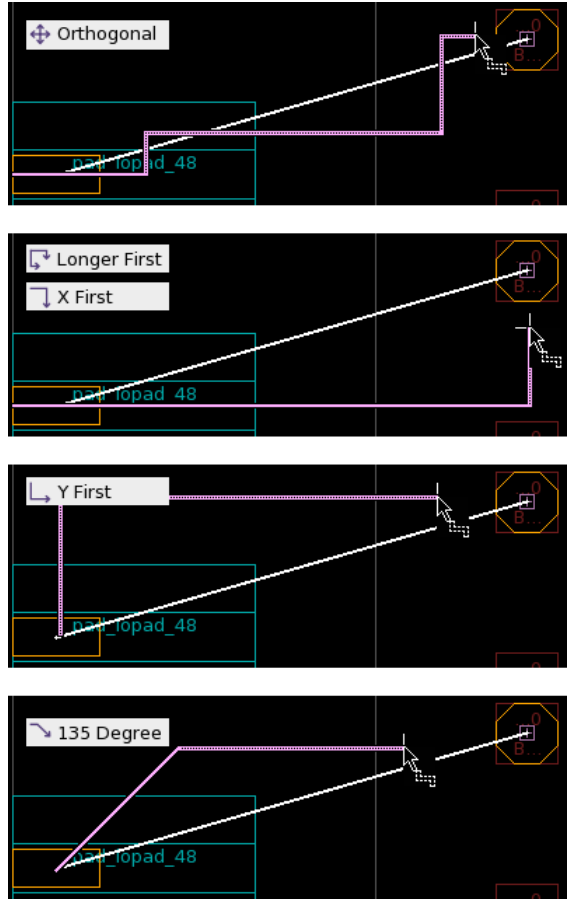
\includegraphics[width=0.92\textwidth]{gui-fig-164.png}
\caption{Create RDL 绘制模式}
\label{fig:gui-164}
\end{figure}

\begin{enumerate}
  \setcounter{enumi}{4}
  \item 单击管脚、端口或线网连接，开始布线。
  \item 单击以完成一段布线，并开始新的一段。
  \item 按 Enter 完成布线。
\end{enumerate}

\subsection{录制并回放 Create Route 操作}
\subsubsection*{Recording and Replaying Create Route Actions}

Create Route 与 Create RDL 工具支持录制功能，用来捕获创建布线时的鼠标操作，并保存到 Script Editor。脚本可以存到磁盘，以后再运行；也可以直接从 Script Editor 运行。录制功能可以配置为容忍管脚位置的小幅变化，从而在设计做过小改动之后重新创建布线。

要创建布线并启用录制：
\begin{enumerate}
  \item 选择 \textbf{Create > Route}、单击 Create Route 按钮，或按 Shift+R，启动 Create Route 工具。选择 \textbf{Create > RDL}，或单击 Create RDL 按钮，启动 Create RDL 工具。
  \item （可选）在工具栏中设置所需的布线选项。
  \item （可选）若预计重新创建布线时，布线中的管脚或线段坐标会发生变化，单击 More，并在 Log/replay coordinates 部分启用 Relative to nets。启用后，工具捕获的是相对整条布线包围盒的坐标，而不是绝对坐标。若要把脚本用于在设计的另一区域创建布线，本选项很有用。
  \item 在 Create Route 工具的工具栏上单击 Record 按钮。
  \item 单击起点、创建线段并结束布线，从而创建该布线。
  \item 布线完成后，打开 Script Editor，单击 Save As 按钮，把脚本保存到文件。
\end{enumerate}

创建线段时，Create Route 工具把操作捕获到 Script Editor。录制功能捕获的示例脚本如下：
\begin{lstlisting}
...
# Info : recording session started
...
gui_mouse_tool -window [gui_get_current_window -types Layout -mru] \
   -start CreateRouteTool
set_edit_setting -default
set_snap_setting -default
...
gui_set_mouse_tool_option -tool CreateRouteTool -all -default
gui_set_mouse_tool_option -tool CreateRouteTool \
   -option {BundleOrNetNames} \
   -value {net2[127] net2[126] net2[125] net2[124]}
...
gui_mouse_tool -window [gui_get_current_window -types Layout -mru] \
   -add_point {455.756 907.825} -scale 0.02
gui_mouse_tool -window [gui_get_current_window -types Layout -mru] \
   -add_point {568.946 1194.223} -scale 5.6331
...
gui_mouse_tool -window [gui_get_current_window -types Layout -mru] -apply
gui_mouse_tool -window [gui_get_current_window -types Layout -mru] -abort
...
# Info : recording session ended
\end{lstlisting}

要重新创建该布线，在 Script Editor 中单击 Run Script 运行脚本。也可以把脚本保存到文件，再用 \cmd{source} 命令执行该脚本。

% ============================================================
\section{对布线做交互式设计规则检查}
\subsection*{Performing Interactive Design Rule Checking on Routes}
\label{sec:gui-route-drc}

GUI 提供两种交互式设计规则检查：
\begin{itemize}
  \item Editor DRC
  \item ICV Live
\end{itemize}

\begin{seeAlsoBox}
Editor DRC 工具的进一步说明，见第~\ref{sec:gui-editor-drc}~节「用 Editor DRC 工具诊断设计规则违例」。ICV Live 功能见 \textit{IC Compiler II Implementation User Guide} 中的 Checking Signoff Design Rules Interactively in the GUI。
\end{seeAlsoBox}

\subsection{用 Editor DRC 工具诊断设计规则违例}
\subsubsection*{Diagnosing Design Rule Violations Using the Editor DRC tool}
\label{sec:gui-editor-drc}

版图视图（layout view）提供 Editor DRC 工具，用来识别并诊断交互编辑操作引起的 DRC 违例。Editor DRC 工具检测设计规则违例，在当前版图视图中显示错误形状，并把违例记入 Editor DRC 错误数据文件。

\begin{noteBox}
Editor DRC 工具只做快速检查，并按工艺文件（technology file）中定义的一组 DRC 规则显示错误。Editor DRC 工具不能代替 IC Validator 这类完整的 DRC 工具。
\end{noteBox}

除 Create Route 工具外，下列版图编辑工具也与 Editor DRC 工具配合使用：
\begin{itemize}
  \item Copy Objects 工具
  \item Create Fill 工具
  \item Create RDL 工具
  \item Create Shape 工具
  \item Create Terminal 工具
  \item Create Via 工具
  \item Quick Connect 工具
  \item Stretch Connected 工具
  \item Stretch 工具
\end{itemize}

\subsection{交互验证布线编辑}
\subsubsection*{Verifying Route Edits Interactively}

要为交互编辑操作启用或关闭 Editor DRC 工具，单击工具栏上的 DRC 按钮，并选择 DRC enabled。

为交互编辑操作启用 Editor DRC 工具后，若检测到违例，工具立即给出可视反馈。版图视图为每种违例显示不同的视觉提示。

Editor DRC 工具支持对下列类型的对象做规则检查：
\begin{itemize}
  \item 水平与垂直的线网形状和用户形状（user shape），包括线、通孔、通孔阵列（via array）、路径（path）、多边形（polygon）与矩形（rectangle）
  \item 端口形状与端子（terminal）
  \item 标准单元（standard cell）、硬宏（hard macro）、软宏（soft macro）与黑盒（black box）
  \item 布线阻挡（routing blockage）
\end{itemize}

\subsection{验证已编辑的线网}
\subsubsection*{Verifying Edited Nets}

要检查所选线网是否存在 Editor DRC 工具违例：
\begin{enumerate}
  \item 选择需要检查的一根或多根线网。
  \item 选择 \textbf{Edit > DRC > Run DRC on Selected Shapes}。也可以使用 \cmd{gui\_check\_drc\_errors} 命令。
\end{enumerate}

若发现错误，工具创建错误数据，并打开 Error Browser 显示这些错误数据。

\subsection{设置 Editor DRC 选项}
\subsubsection*{Setting Editor DRC Options}

Editor DRC 工具按工艺文件中定义的一组 DRC 规则做规则检查。交互编辑工具使用 Editor DRC 工具，检测交互编辑期间出现的布线设计规则违例。可以设置工具能够检测的最大违例数，并控制检测到违例时工具是否自动打开错误浏览器并加载错误。

当支持 Editor DRC 的工具处于活动状态时，单击工具栏上的 DRC 按钮，即可设置 Editor DRC 工具选项。

在 Editor DRC options 对话框中更改选项后，更改立即作用于全部已打开版图视图中所有适用的工具。若在 Application Preferences 对话框中启用了 GUI 命令输出日志，工具还会在控制台（console）日志视图与历史视图中显示 \cmd{set\_edrc\_setting} 命令，从而记录这次更改。

\subsection{查看 Editor DRC 报告的错误}
\subsubsection*{Examining Errors Reported by Editor DRC}

Editor DRC 工具检测到设计规则违例时，在当前版图视图中显示错误形状，把错误记入 Editor DRC 错误视图，并自动把错误信息加载到错误浏览器，如图~\ref{fig:gui-165} 所示。

\begin{figure}[htbp]
\centering
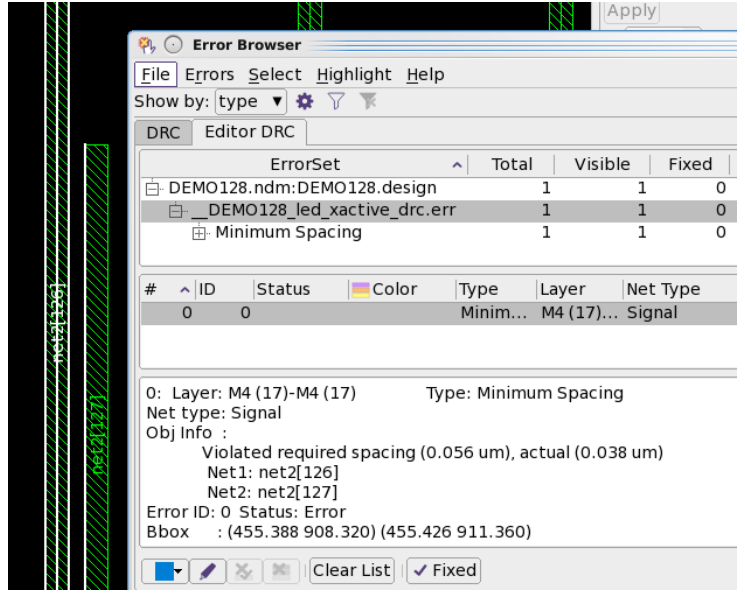
\includegraphics[width=0.92\textwidth]{gui-fig-165.png}
\caption{Editor DRC}
\label{fig:gui-165}
\end{figure}

错误视图包含两类违例记录：交互编辑期间检测到的违例，以及对所选形状运行检查时检测到的违例。修正违例、撤销引起违例的编辑操作、关闭用于检测该违例的设计规则检查，或在错误浏览器中删除错误时，Editor DRC 工具会更新错误数据。

Editor DRC 错误视图与当前设计关联。在关闭设计或更改当前设计之前，它一直打开并加载在错误浏览器中。保存或关闭设计时，工具不保存该错误视图。若关闭当前设计，Editor DRC 工具会关闭错误视图，并从错误浏览器中去掉这些错误。

% ============================================================
\section{用 Tcl 命令或 GUI 创建布线主干}
\subsection*{Creating Route Trunks With Tcl Commands or GUI}

IC Compiler II GUI 支持用 Tcl 命令为指定线网和线束创建布线主干（route trunk）。使用 \cmd{create\_trunk}、\cmd{create\_trunk\_shared\_track}、\cmd{create\_trunk\_pin\_to\_trunk}、\cmd{create\_trunk\_pin\_to\_pin} 与 \cmd{create\_trunk\_topology} 命令创建主干线段与连接，如本节所述。

\subsection{沿一个方向创建布线段}
\subsubsection*{Creating Route Segments in One Direction}

要在单一金属层上沿一个方向创建布线主干，按如下方式使用 \cmd{create\_trunk} 命令：
\begin{lstlisting}
icc2_shell> set nets [get_nets {net1 net2 net3 net4}]
icc2_shell> create_trunk -nets $nets -layer M3 \
   -gravity percentage -percentage 25
\end{lstlisting}

该命令为 \opt{-nets} 选项指定的每根线网或每个线束创建一条布线段。本例中，\opt{-gravity percentage} 指定布线段如何与这些线网的包围盒对齐。\opt{-percentage 25} 指定第一条布线段放在包围盒底边再加上包围盒高度 25\% 的位置。百分比取 25、50 与 75 时的不同布线结果如图~\ref{fig:gui-166} 所示。

\begin{figure}[htbp]
\centering
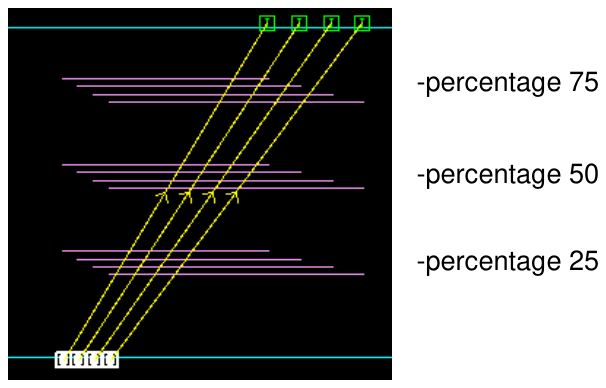
\includegraphics[width=0.92\textwidth]{gui-fig-166.png}
\caption{创建主干}
\label{fig:gui-166}
\end{figure}

为 \cmd{create\_trunk} 命令指定下列选项，以控制布线的创建方式。
\begin{itemize}
  \item 用 \opt{-direction horizontal | vertical} 指定该层的布线方向。默认情况下，命令沿首选方向（preferred direction）创建布线。
  \item 指定 \opt{-gravity driver}，使布线与线网的驱动端对齐。指定 \opt{-gravity load}，使布线与线网的负载端对齐。
  \item 用 \opt{-track\_numbers}、\opt{-track\_coords}、\opt{-track\_step} 与 \opt{-track\_ref\_bbox} 在线网包围盒内的指定轨道上创建布线。例如，要在从 (50,50) 到 (100,100) 的包围盒内创建布线，并从盒内第二条轨道开始，指定下列命令：
\begin{lstlisting}
icc2_shell> create_trunk -nets $nets -layer M3 \
   -track_ref_bbox {{50 50} {100 100}} -track_numbers 2
\end{lstlisting}
  \item 用 \opt{-avoid\_obstructions} 把布线放到下一条没有障碍（obstruction）的可用轨道上。默认情况下，若发现障碍，命令发出警告并跳过该线网。
  \item 用 \opt{-do\_not\_check\_shorts} 关闭对短路（short）与障碍的检查，并预览布线。
\end{itemize}

使用 \opt{-do\_not\_check\_shorts} 与 \opt{-avoid\_obstructions} 得到的版图结果如图~\ref{fig:gui-167} 所示。

\begin{figure}[htbp]
\centering
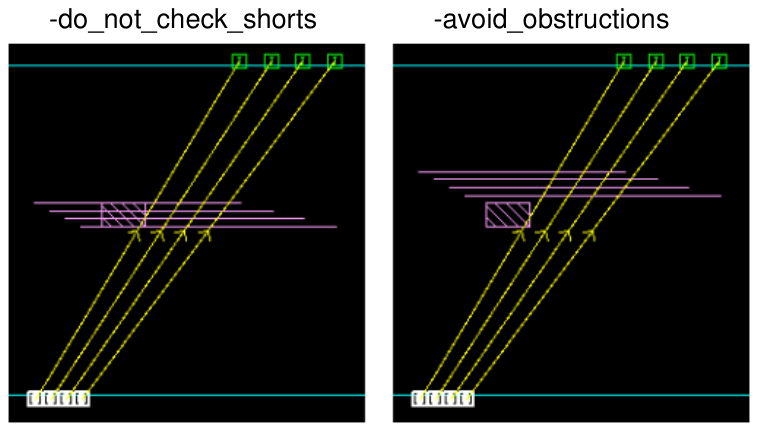
\includegraphics[width=0.92\textwidth]{gui-fig-167.png}
\caption{忽略障碍与短路，以及避开障碍}
\label{fig:gui-167}
\end{figure}

\begin{itemize}
  \item 用 \opt{-do\_not\_snap\_to\_track} 避免把布线吸附到轨道。
  \item 用 \opt{-num\_wires} 为每根线网创建不止一条布线。
  \item 用 \opt{-width} 把布线限制在特定轨道宽度上。默认情况下，布线创建在默认宽度的轨道上。
\end{itemize}

要在 GUI 中于单一金属层上沿一个方向创建布线主干：
\begin{enumerate}
  \item 选择 \textbf{Task > Trunk Routing}。
  \item 在 Trunk Routing 面板中单击 Setup。
  \item 在 Trunk Routing Setup 窗口中单击 \cmd{create\_trunk} 链接。
  \item 指定要为其创建布线主干的线网或线束。
  \item 指定创建布线主干所用的层。
  \item （可选）按需要填写其余字段。
  \item 单击 OK。
\end{enumerate}

\begin{figure}[htbp]
\centering
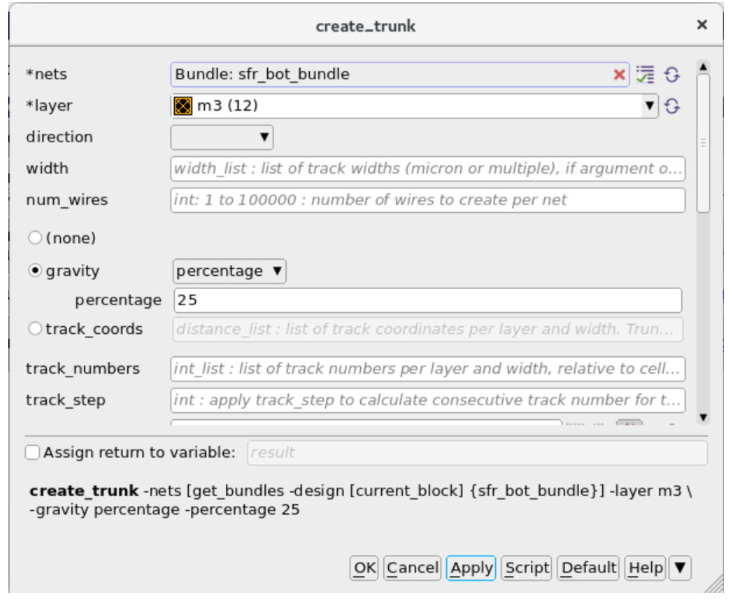
\includegraphics[width=0.92\textwidth]{gui-fig-168.png}
\caption{create\_trunk 命令的 GUI}
\label{fig:gui-168}
\end{figure}

\begin{figure}[htbp]
\centering
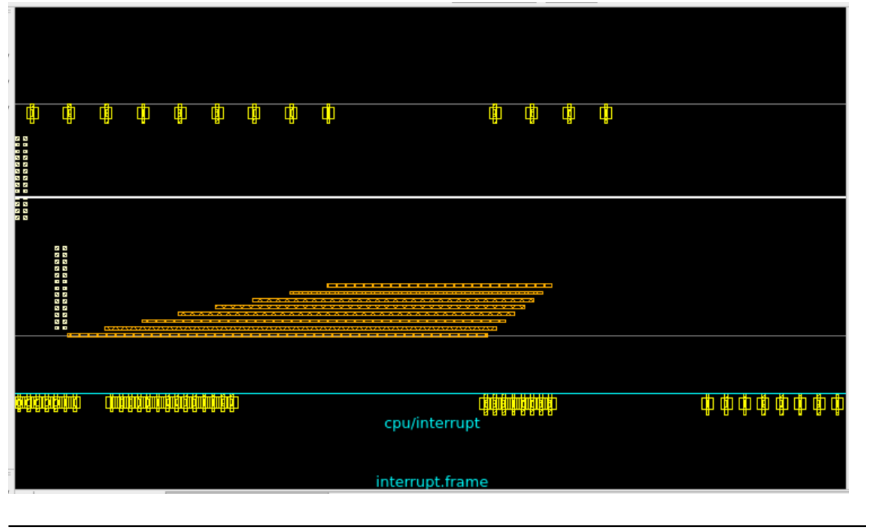
\includegraphics[width=0.92\textwidth]{gui-fig-169.png}
\caption{create\_trunk 命令的结果}
\label{fig:gui-169}
\end{figure}

\subsection{在同一轨道上沿一个方向创建布线段}
\subsubsection*{Creating Route Segments on the Same Track in One Direction}

要在同一条轨道上沿一个方向创建布线主干，按如下方式使用 \cmd{create\_trunk\_shared\_track} 命令：
\begin{lstlisting}
icc2_shell> create_trunk_shared_track -nets {sfr_small_bundle} -layer m3 \
   -track_coord 175 -width {0.4 0.6}
\end{lstlisting}

该命令为 \opt{-nets} 选项指定的每根线网创建一条布线段。本例中，\opt{-track\_coord} 指定决定布线起点的 x 或 y 坐标，并吸附到最近的轨道。\opt{-width} 指定放置这些布线的轨道宽度列表。

\begin{figure}[htbp]
\centering
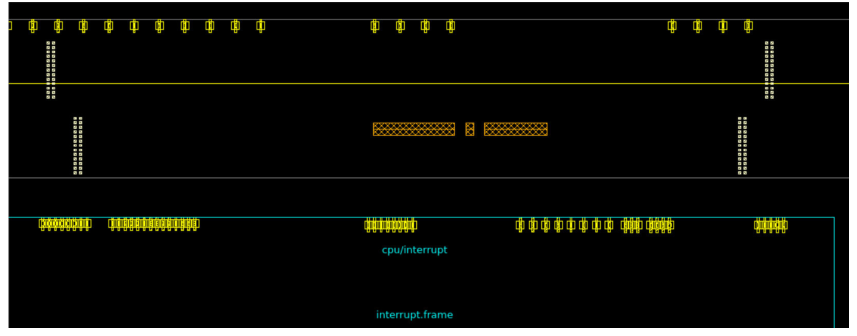
\includegraphics[width=0.92\textwidth]{gui-fig-170.png}
\caption{在同一轨道上沿一个方向创建布线段}
\label{fig:gui-170}
\end{figure}

为 \cmd{create\_trunk\_shared\_track} 命令指定下列选项，以控制布线的创建方式。
\begin{itemize}
  \item 用 \opt{-layer} 指定把管脚连接到布线所用的层。命令沿指定层的首选方向创建布线，并跳过非首选方向上的连接。
  \item 用 \opt{-direction horizontal | vertical} 指定该层的布线方向。默认情况下，命令沿首选方向创建布线。
  \item 用 \opt{-track\_numbers}、\opt{-track\_coords} 与 \opt{-track\_ref\_bbox} 在线网包围盒内的指定轨道上创建布线。
  \item 用 \opt{-avoid\_obstructions} 把布线放到下一条没有障碍的可用轨道上。默认情况下，若发现障碍，命令发出警告并跳过该线网。
  \item 用 \opt{-do\_not\_check\_shorts} 关闭对短路与障碍的检查，并预览布线。
  \item 用 \opt{-do\_not\_snap\_to\_track} 避免把布线吸附到轨道。
  \item 用 \opt{-track\_freedom} 允许在 \opt{-track\_ref\_bbox} 指定的边界之外，或在由指定线网的管脚连接所定义的包围盒之外创建布线。本选项与 \opt{-avoid\_obstructions} 一起使用。
  \item 用 \opt{-start\_pullback} 从起始管脚一侧缩短布线段，或用 \opt{-stop\_pullback} 在结束管脚一侧缩短布线段。若要把布线段延长而不是缩短，为该距离指定负值。
\end{itemize}

\opt{-start\_pullback} 与 \opt{-stop\_pullback} 既作用于信号，也作用于屏蔽（shielding）。只用 \opt{-shield\_pullback} 为屏蔽指定额外的回拉（pullback）。
\begin{itemize}
  \item 用 \opt{-gap} 在同一条轨道上的主干之间加入间隙。
  \item 用 \opt{-net\_bbox\_override} 指定创建布线段所用的包围盒。指定线网的实际包围盒被忽略，命令也不会尝试连接管脚。
  \item 用 \opt{-of\_cells} 或 \opt{-exclude\_cells} 在计算线网包围盒时包含或排除单元。在多扇出情形下使用这些选项，可以避免不必要的分支。
  \item 用 \opt{-create\_obstruction} 创建布线阻挡，而不创建布线形状。
  \item 用 \opt{-skip\_lib\_cells} 避免在库单元中搜索障碍。本选项与 \opt{-avoid\_obstructions} 一起使用。
  \item 用 \opt{-depth} 指定搜索障碍的层次（hierarchy）深度。默认搜索全部层次。本选项与 \opt{-avoid\_obstructions} 一起使用。
\end{itemize}

要在 GUI 中于同一条轨道上沿一个方向创建布线主干：
\begin{enumerate}
  \item 选择 \textbf{Task > Trunk Routing}。
  \item 在 Trunk Routing 面板中单击 Setup。
  \item 在 Trunk Routing Setup 窗口中单击 \cmd{create\_trunk\_shared\_track} 链接。
  \item 指定要为其创建布线主干的线网或线束。
  \item 指定创建布线主干所用的层。
  \item （可选）按需要填写其余字段。
  \item 单击 OK。
\end{enumerate}

\begin{figure}[htbp]
\centering
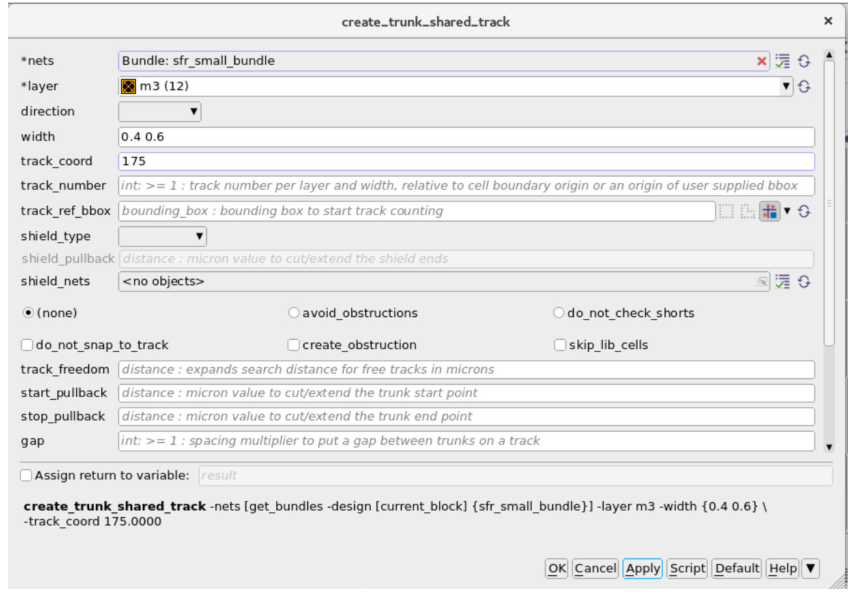
\includegraphics[width=0.92\textwidth]{gui-fig-171.png}
\caption{create\_trunk\_shared\_track 命令的 GUI}
\label{fig:gui-171}
\end{figure}

\begin{figure}[htbp]
\centering
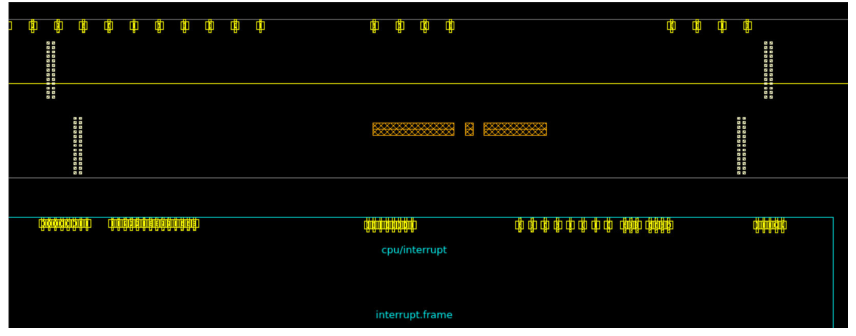
\includegraphics[width=0.92\textwidth]{gui-fig-172.png}
\caption{create\_trunk\_shared\_track 命令的结果}
\label{fig:gui-172}
\end{figure}

\subsection{从管脚连接到已有布线段}
\subsubsection*{Creating Routes From Pins to Existing Route Segments}

要在管脚与已有布线段之间创建布线，按如下方式使用 \cmd{create\_trunk\_pin\_to\_trunk} 命令：
\begin{lstlisting}
icc2_shell> create_bundle b1 [get_nets {net1 net2 net3 net4}]
icc2_shell> create_trunk_pin_to_trunk -nets b1
\end{lstlisting}

该命令在已有布线主干与该主干上线网所关联的最近管脚之间创建一条布线段，如图~\ref{fig:gui-173} 所示。本例中，布线创建在与管脚相同的层上。

\begin{figure}[htbp]
\centering
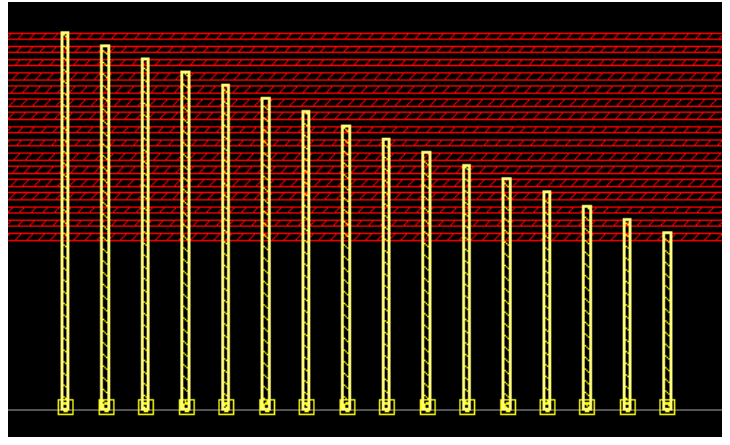
\includegraphics[width=0.92\textwidth]{gui-fig-173.png}
\caption{把管脚连接到已有布线}
\label{fig:gui-173}
\end{figure}

为 \cmd{create\_trunk\_pin\_to\_trunk} 命令指定下列选项，以控制布线的创建方式。
\begin{itemize}
  \item 用 \opt{-layer} 指定把管脚连接到布线所用的层。命令沿指定层的首选方向创建布线，并跳过非首选方向上的连接。
  \item 用 \opt{-direction horizontal | vertical} 沿指定方向创建布线段。另一方向上的连接被跳过。
  \item 用 \opt{-do\_not\_snap\_to\_track} 避免把布线吸附到轨道。
  \item 用 \opt{-avoid\_obstructions} 把布线放到下一条没有障碍的可用轨道上。默认情况下，若发现障碍，命令发出警告并跳过该线网。
  \item 用 \opt{-do\_not\_check\_shorts} 关闭对短路与障碍的检查，并预览布线。
  \item 用 \opt{-cluster\_proximity} 减少从主干创建的布线形状数量。用本选项指定一个以微米为单位的范围，把该范围内单独的管脚到主干形状合并为单一形状。命令会从主干创建布线段，但可能不完成到管脚的连接。
\end{itemize}

为聚类邻近距离指定三个不同值之后的版图结果如图~\ref{fig:gui-174} 所示。

\begin{figure}[htbp]
\centering
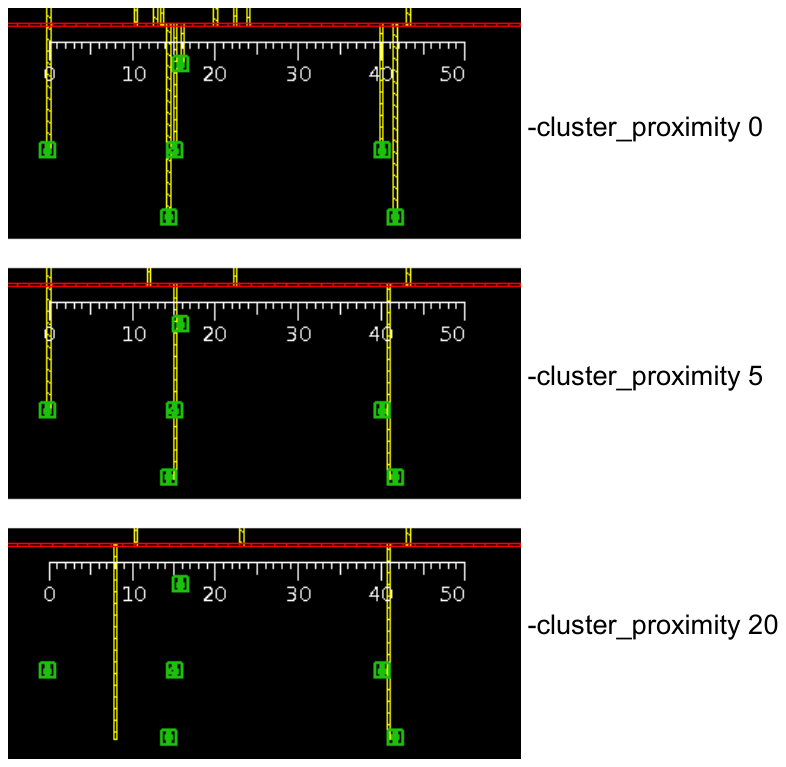
\includegraphics[width=0.92\textwidth]{gui-fig-174.png}
\caption{聚类邻近距离}
\label{fig:gui-174}
\end{figure}

要补上缺少的连接，再次运行 \cmd{create\_trunk\_pin\_to\_trunk}，并指定正交方向上的层。下面的示例先创建垂直布线，然后再次调用 \cmd{create\_trunk\_pin\_to\_trunk}，以完成到管脚的连接。
\begin{lstlisting}
icc2_shell> create_trunk_pin_to_trunk -nets $nets -layer METAL2 \
   -cluster_proximity 40
icc2_shell> create_trunk_pin_to_trunk -nets $nets -layer METAL3
\end{lstlisting}

要在 GUI 中于管脚与已有布线段之间创建布线：
\begin{enumerate}
  \item 选择 \textbf{Task > Trunk Routing}。
  \item 在 Trunk Routing 面板中单击 Setup。
  \item 在 Trunk Routing Setup 窗口中单击 \cmd{create\_trunk\_pin\_to\_trunk} 链接。
  \item 指定要为其创建布线主干的线网。
  \item （可选）按需要填写其余字段。
  \item 单击 OK。
\end{enumerate}

\begin{figure}[htbp]
\centering
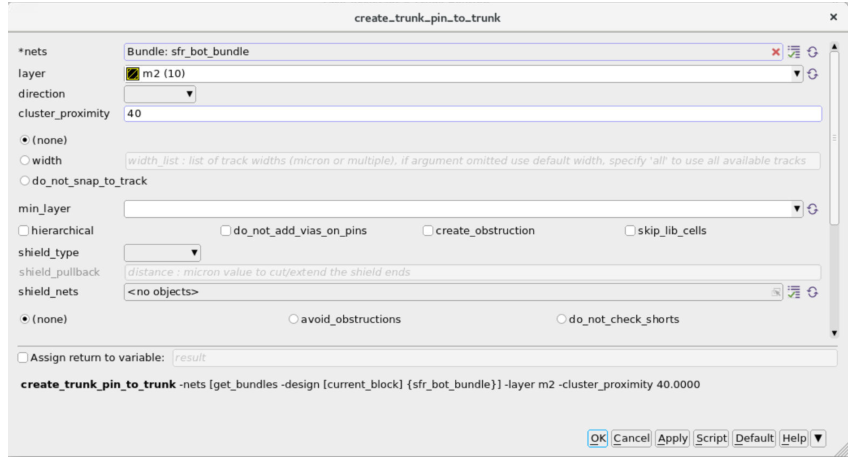
\includegraphics[width=0.92\textwidth]{gui-fig-175.png}
\caption{create\_trunk\_pin\_to\_trunk 命令的 GUI}
\label{fig:gui-175}
\end{figure}

\begin{figure}[htbp]
\centering
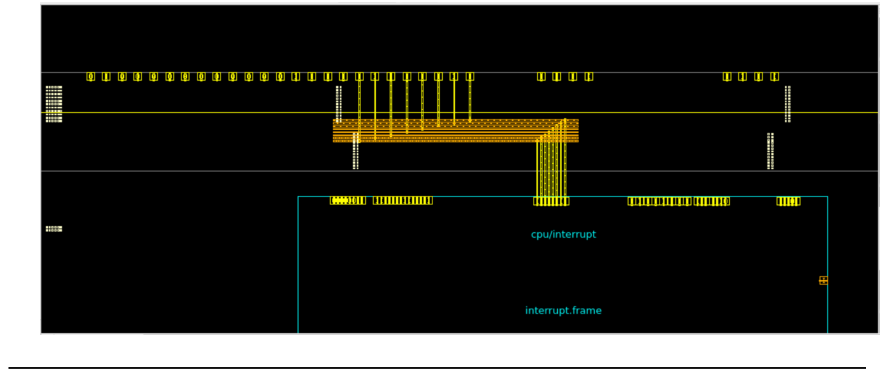
\includegraphics[width=0.92\textwidth]{gui-fig-176.png}
\caption{create\_trunk\_pin\_to\_trunk 命令的结果}
\label{fig:gui-176}
\end{figure}

\subsection{从管脚到管脚创建布线}
\subsubsection*{Creating Routes From Pin to Pin}

要在管脚之间创建布线段，按如下方式使用 \cmd{create\_trunk\_pin\_to\_pin} 命令：
\begin{lstlisting}
icc2_shell> create_bundle b1 [get_nets {net1 net2 net3 net4}]
icc2_shell> create_trunk_pin_to_pin -nets b1 \
   -extensions {0.67 1.0 0.33} -layer_legs {M4 M3 M4}
\end{lstlisting}

该命令产生的版图结果如图~\ref{fig:gui-177} 所示。

\begin{figure}[htbp]
\centering
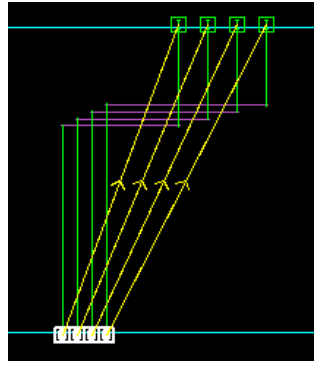
\includegraphics[width=0.92\textwidth]{gui-fig-177.png}
\caption{管脚到管脚的布线主干}
\label{fig:gui-177}
\end{figure}

本例中，\opt{-extensions} 指定各布线段的相对长度，从驱动管脚开始，到负载管脚结束。要反转某一段的方向，为延伸值指定负数。要从目标管脚开始布线，见下面列表中对 \opt{-start\_from} 的说明。各段对应的层用 \opt{-layer\_legs} 指定。

为 \cmd{create\_trunk\_pin\_to\_pin} 命令指定下列选项，以控制布线的创建方式。
\begin{itemize}
  \item 用 \opt{-layer\_legs} 指定给定层所用的具体轨道宽度。例如，下列命令只把布线放在 M2 与 M3 上宽度为 0.4 或 0.8 的轨道上。要使用任意可用轨道宽度，把 \cmd{\{0.4 0.8\}} 换成 \cmd{all} 参数。默认情况下，命令只把布线放在默认宽度的轨道上。
\begin{lstlisting}
icc2_shell> create_trunk_pin_to_pin -nets $nets \
   -layer_legs {{METAL2 {0.4 0.8}} {METAL3 {0.4 0.8}}} \
   -extensions {1 1}
\end{lstlisting}
  \item 用 \opt{-extensions} 指定每一段的长度。该选项接受一个延伸值列表，列表中的每个元素指定布线中一段的长度。延伸值可以指定为线网包围盒的分数、线网包围盒的百分比、以微米为单位的距离，或用户定义的单位。
  \item 用 \opt{-layer\_legs} 与一个层列表一起指定每一段所用的层。每一层对应 \opt{-extensions} 所指定的一段。
  \item 用 \opt{-net\_bbox\_override} 指定创建布线段所用的包围盒。指定线网的实际包围盒被忽略，命令也不会尝试连接管脚。
  \item 用 \opt{-start\_from} 指定开始布线的管脚的相对位置。
\end{itemize}

在下面的示例中，第一条命令从位于图下方的源管脚开始布线，得到左侧的版图结果；第二条命令从位于图上方的目标管脚开始布线，得到右侧的版图结果。
\begin{lstlisting}
icc2_shell> create_trunk_pin_to_pin -nets b4 \
   -extensions {0.25 1.0 0.75} -layer_legs {M4 M3 M4}
icc2_shell> create_trunk_pin_to_pin -nets b4 \
   -extensions {0.25 1.0 0.75} -layer_legs {M4 M3 M4} \
   -start_from high_y
\end{lstlisting}

\begin{figure}[htbp]
\centering
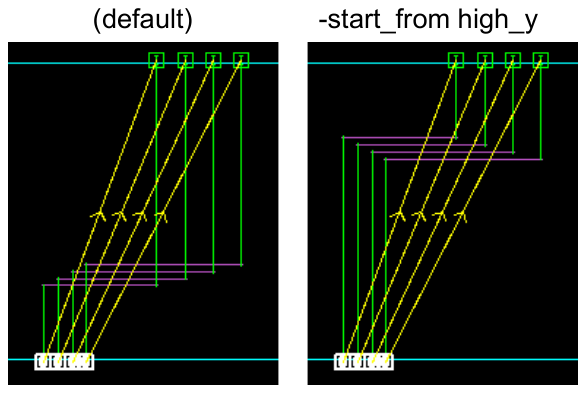
\includegraphics[width=0.92\textwidth]{gui-fig-178.png}
\caption{起始位置}
\label{fig:gui-178}
\end{figure}

\begin{itemize}
  \item 用 \opt{-do\_not\_snap\_to\_track} 避免把布线吸附到轨道。
  \item 用 \opt{-do\_not\_check\_shorts} 关闭对短路与障碍的检查，并预览布线。
  \item 用 \opt{-start\_pullback} 从起始管脚一侧缩短布线段，或用 \opt{-stop\_pullback} 在结束管脚一侧缩短布线段。若要把布线段延长而不是缩短，为该距离指定负值。
\end{itemize}

\opt{-start\_pullback} 与 \opt{-stop\_pullback} 既作用于信号，也作用于屏蔽。只用 \opt{-shield\_pullback} 为屏蔽指定额外的回拉。

要在 GUI 中于管脚之间创建布线段：
\begin{enumerate}
  \item 选择 \textbf{Task > Trunk Routing}。
  \item 在 Trunk Routing 面板中单击 Setup。
  \item 在 Trunk Routing Setup 窗口中单击 \cmd{create\_trunk\_pin\_to\_pin} 链接。
  \item 指定要为其创建布线主干的线网或线束。
  \item 指定创建布线主干所用的层。
  \item 在 extensions 文本框中指定布线的相对长度。
  \item （可选）按需要填写其余字段。
  \item 单击 OK。
\end{enumerate}

\begin{figure}[htbp]
\centering
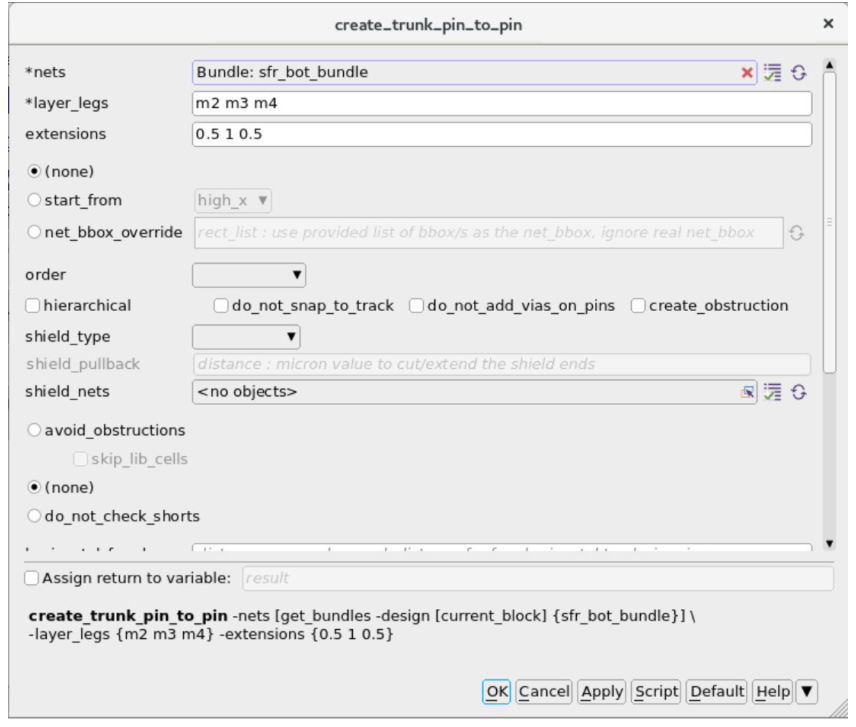
\includegraphics[width=0.92\textwidth]{gui-fig-179.png}
\caption{create\_trunk\_pin\_to\_pin 命令的 GUI}
\label{fig:gui-179}
\end{figure}

\begin{figure}[htbp]
\centering
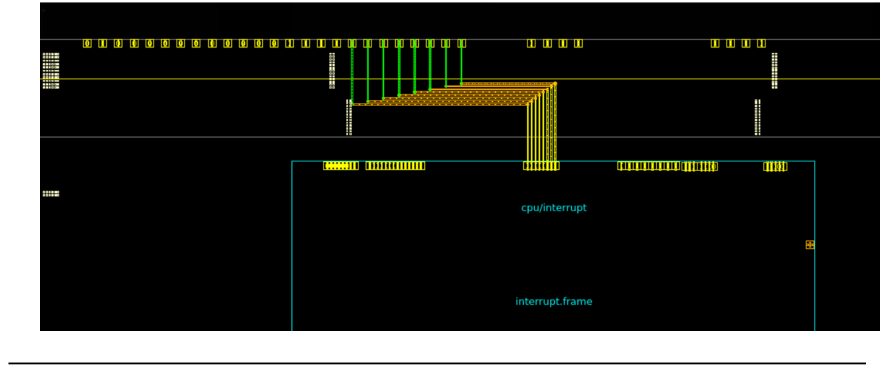
\includegraphics[width=0.92\textwidth]{gui-fig-180.png}
\caption{create\_trunk\_pin\_to\_pin 命令的结果}
\label{fig:gui-180}
\end{figure}

\subsection{从拓扑边创建布线}
\subsubsection*{Creating Routes From Topology Edges}

要从拓扑边（topology edge）创建布线，按如下方式使用 \cmd{create\_trunk\_topology} 命令：
\begin{lstlisting}
icc2_shell> set shape_layers {{m2 50% 0} {m3 100% 0} {m4 50% 0}}
icc2_shell> create_topology_plan -name TP1 -objects \
   [get_bundles sfr_bot_bundle]
icc2_shell> create_topology_node -plan TP1 -name N1 -constraint_type bbox \
   -objects [get_ports sfr_data_out* ]
icc2_shell> create_topology_node -plan TP1 -name N2 \
   -constraint_type bbox -objects [get_pins cpu/interrupt/sfr_data_out* ]
icc2_shell> create_topology_edge -name E12 -plan TP1 \
   -nodes {TP1/N1 TP1/N2} -shape_layers $shape_layers \
   -objects [get_nets sfr_data_out*]
icc2_shell> create_trunk_topology -edge TP1/E12
\end{lstlisting}

上面这一组命令创建的版图结果如图~\ref{fig:gui-181} 所示。

\begin{figure}[htbp]
\centering
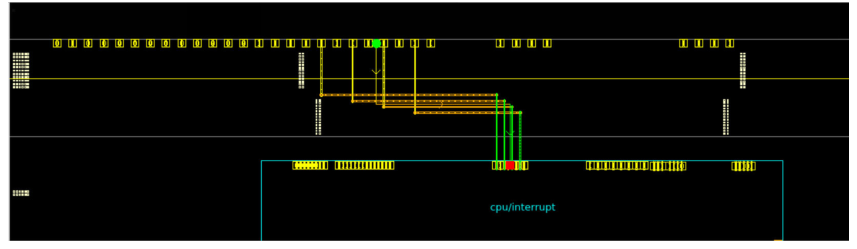
\includegraphics[width=0.92\textwidth]{gui-fig-181.png}
\caption{从拓扑边布线}
\label{fig:gui-181}
\end{figure}

本例中，\opt{-edge} 指定要为其创建布线的拓扑边名称。

为 \cmd{create\_trunk\_topology} 命令指定下列选项，以控制布线的创建方式。
\begin{itemize}
  \item 用 \opt{-plan} 指定要为其创建布线的拓扑规划（topology plan）名称或集合。
  \item 用 \opt{-avoid\_obstructions} 把布线放到下一条没有障碍的可用轨道上。默认情况下，若发现障碍，命令发出警告并跳过该线网。
  \item 用 \opt{-do\_not\_check\_shorts} 关闭对短路与障碍的检查，并预览布线。
  \item 用 \opt{-do\_not\_snap\_to\_track} 避免把布线吸附到轨道。
  \item 用 \opt{-do\_not\_add\_vias\_on\_pins} 避免在管脚上添加通孔。
  \item 用 \opt{-horizontal\_freedom} 或 \opt{-vertical\_freedom} 在水平或垂直方向上扩大布线可以挪动的区域。
  \item 用 \opt{-start\_pullback} 从起始管脚一侧缩短布线段，或用 \opt{-stop\_pullback} 在结束管脚一侧缩短布线段。若要把布线段延长而不是缩短，为该距离指定负值。
\end{itemize}

\opt{-start\_pullback} 与 \opt{-stop\_pullback} 既作用于信号，也作用于屏蔽。只用 \opt{-shield\_pullback} 为屏蔽指定额外的回拉。
\begin{itemize}
  \item 用 \opt{-skip\_lib\_cells} 避免在库单元中搜索障碍。本选项与 \opt{-avoid\_obstructions} 一起使用。
\end{itemize}

要在 GUI 中从拓扑边创建布线段：
\begin{enumerate}
  \item 选择 \textbf{Task > Trunk Routing}。
  \item 在 Trunk Routing 面板中单击 Setup。
  \item 在 Trunk Routing Setup 窗口中单击 \cmd{create\_trunk\_topology} 链接。
  \item 指定要为其创建布线的拓扑规划名称或边。
  \item （可选）按需要填写其余字段。
  \item 单击 OK。
\end{enumerate}

\begin{figure}[htbp]
\centering
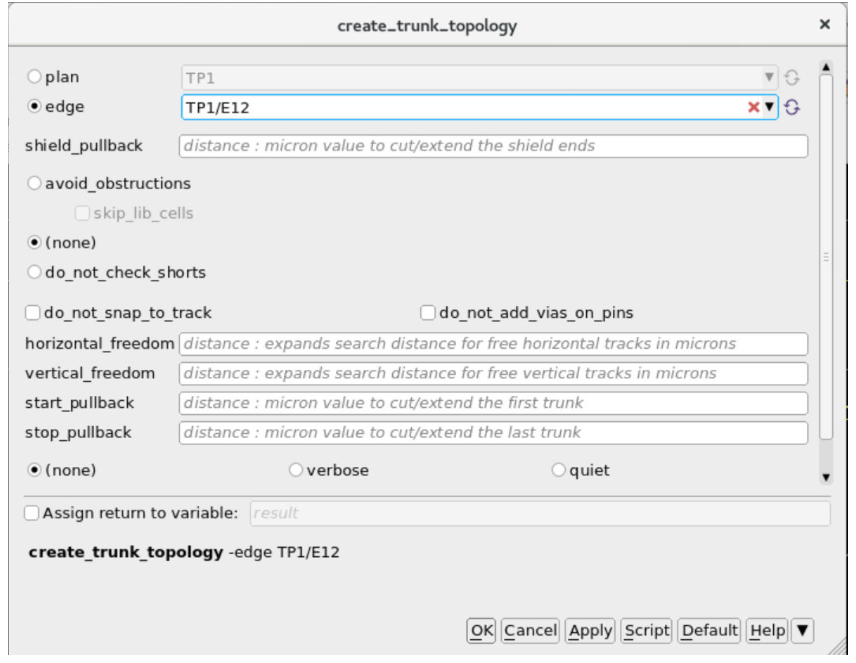
\includegraphics[width=0.92\textwidth]{gui-fig-182.png}
\caption{create\_trunk\_topology 命令的 GUI}
\label{fig:gui-182}
\end{figure}

\begin{figure}[htbp]
\centering
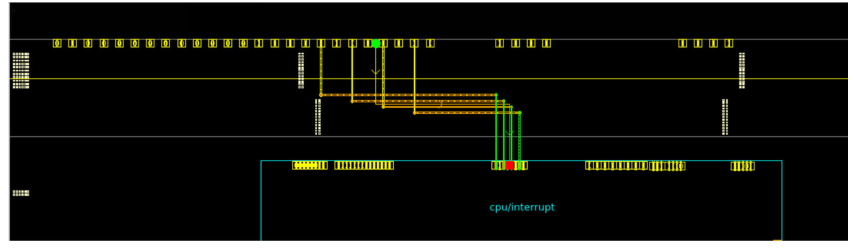
\includegraphics[width=0.92\textwidth]{gui-fig-183.png}
\caption{create\_trunk\_topology 命令的结果}
\label{fig:gui-183}
\end{figure}

\subsection{布线区域包围盒}
\subsubsection*{Routing Area Bounding Box}

默认情况下，\cmd{create\_trunk} 与 \cmd{create\_trunk\_pin\_to\_pin} 在由源管脚与目标管脚形成的包围盒内创建布线，如图~\ref{fig:gui-184} 所示。

\begin{figure}[htbp]
\centering
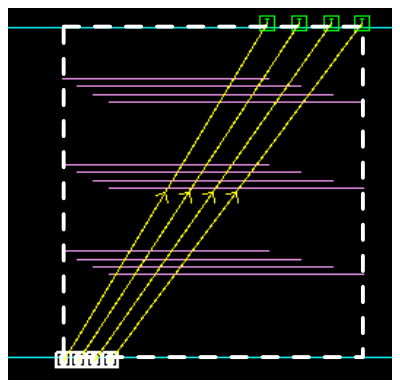
\includegraphics[width=0.92\textwidth]{gui-fig-184.png}
\caption{布线主干的默认包围盒}
\label{fig:gui-184}
\end{figure}

要在指定包围盒内创建布线主干，为 \cmd{create\_trunk} 与 \cmd{create\_trunk\_pin\_to\_pin} 指定 \opt{-net\_bbox\_override}。下面的示例在由 (100,100) 与 (200,200) 围成的盒子内，为 \cmd{net1} 与 \cmd{net2} 创建布线主干。
\begin{lstlisting}
icc2_shell> create_trunk -nets {net1 net2} -layer METAL3 \
   -net_bbox_override {{100 100} {200 200}}
\end{lstlisting}

\subsection{屏蔽线网}
\subsubsection*{Shielding Nets}

可以用 \opt{-shield\_nets} 与 \opt{-shield\_type} 选项，配合 \cmd{create\_trunk}、\cmd{create\_trunk\_pin\_to\_trunk} 或 \cmd{create\_trunk\_pin\_to\_pin} 创建屏蔽线网。\opt{-shield\_type} 支持布线上的全屏蔽（full）、部分屏蔽（partial）或端帽屏蔽（cap）。屏蔽线网在各线网之间共享。屏蔽线网的顺序与位置相对 x 轴和 y 轴。因此，低端屏蔽线网总是从较低的 x 或 y 位置开始，高端屏蔽线网从较高的 x 或 y 位置开始。工具支持全交错屏蔽（full interleaved shielding）与半交错屏蔽（half interleaved shielding）。

\opt{-start\_pullback} 与 \opt{-stop\_pullback} 既作用于信号，也作用于屏蔽。只用 \opt{-shield\_pullback} 为屏蔽指定额外的回拉。

图~\ref{fig:gui-185} 给出没有屏蔽线网时的默认版图结果，以及运行下列命令创建屏蔽线网之后的版图结果。由 \cmd{\$nets} 指定的非屏蔽线网被高亮，供对照。
\begin{lstlisting}
icc2_shell> create_trunk -nets $nets -layer M3 \
   -shield_nets VDD -shield_type full
\end{lstlisting}

\begin{figure}[htbp]
\centering
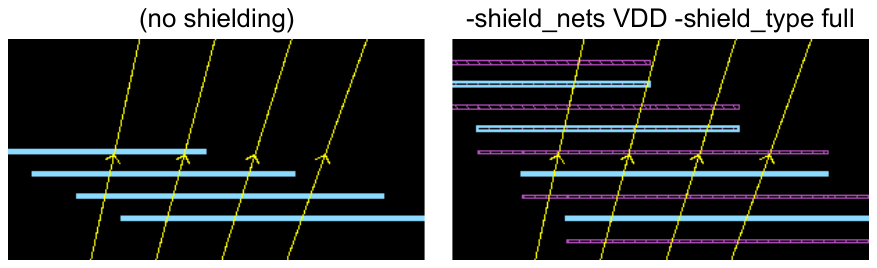
\includegraphics[width=0.92\textwidth]{gui-fig-185.png}
\caption{屏蔽线网}
\label{fig:gui-185}
\end{figure}

图~\ref{fig:gui-186} 与图~\ref{fig:gui-187} 给出全屏蔽 \cmd{\{VCC VSS\}} 的共享线网示例，分别采用河流式拐角（river corner）与交叉式拐角（cross corner）。这两幅图是运行下列命令创建屏蔽线网之后的结果。
\begin{lstlisting}
icc2_shell> create_trunk_pin_to_pin -nets $nets \
   -extensions {0.5 1.0 0.5} -layer_legs {M3 M2 M3} \
   -shield_type full -shield_nets VCC VSS
\end{lstlisting}

\begin{figure}[htbp]
\centering
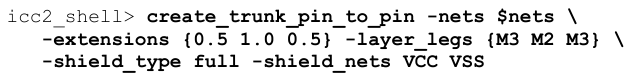
\includegraphics[width=0.92\textwidth]{gui-fig-186.png}
\caption{河流式拐角的全交错屏蔽（VCC 为绿色，VSS 为蓝色）}
\label{fig:gui-186}
\end{figure}

\begin{figure}[htbp]
\centering
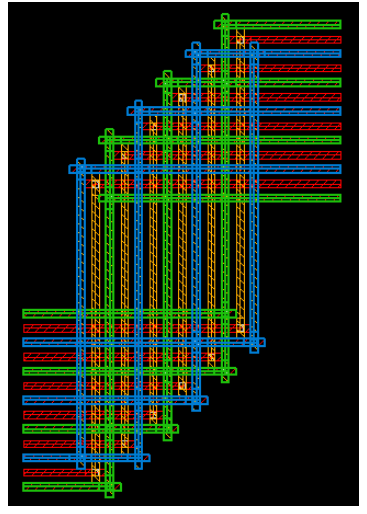
\includegraphics[width=0.92\textwidth]{gui-fig-187.png}
\caption{交叉式拐角的全交错屏蔽（VCC 为绿色，VSS 为蓝色）}
\label{fig:gui-187}
\end{figure}

图~\ref{fig:gui-188} 与图~\ref{fig:gui-189} 给出半屏蔽 \cmd{\{VCC VSS\}} 的共享线网示例，分别采用河流式拐角与交叉式拐角。这两幅图是运行下列命令创建屏蔽线网之后的结果。
\begin{lstlisting}
icc2_shell> create_trunk_pin_to_pin -nets $nets \
   -extensions {0.5 1.0 0.5} -layer_legs {M3 M2 M3} \
   -shield_type half -shield_nets VCC VSS
\end{lstlisting}

\begin{figure}[htbp]
\centering
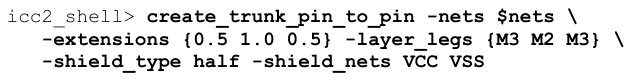
\includegraphics[width=0.92\textwidth]{gui-fig-188.png}
\caption{河流式拐角的半交错屏蔽（VCC 为绿色，VSS 为蓝色）}
\label{fig:gui-188}
\end{figure}

\begin{figure}[htbp]
\centering
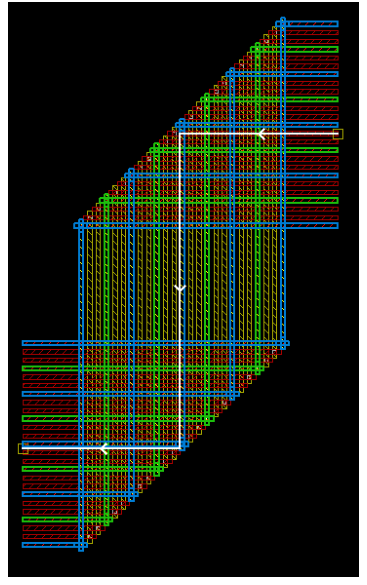
\includegraphics[width=0.92\textwidth]{gui-fig-189.png}
\caption{交叉式拐角的半交错屏蔽（VCC 为绿色，VSS 为蓝色）}
\label{fig:gui-189}
\end{figure}

要使 \cmd{create\_trunk\_pin\_to\_pin} 使用已有的 PG 网格（PG mesh）做屏蔽，需保证 PG 网格线宽与其下方轨道的宽度一致，见图~\ref{fig:gui-190}。

\begin{figure}[htbp]
\centering
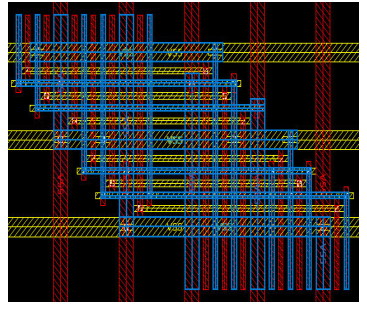
\includegraphics[width=0.92\textwidth]{gui-fig-190.png}
\caption{与地网格共享的全屏蔽 \{VSS\}}
\label{fig:gui-190}
\end{figure}
